\documentclass[12pt, a4paper, twoside, openright]{report}
\usepackage[T1]{fontenc}
\usepackage[utf8]{inputenc}
\usepackage[english]{babel}
\renewcommand{\chaptername}{}
\makeatletter
\renewcommand{\@makechapterhead}[1]{%
  \vspace*{50pt}
  {\parindent \z@ \raggedright \normalfont
    \huge\bfseries \thechapter\quad #1\par\nobreak\vskip 40pt}
}
\makeatother
\usepackage[nottoc]{tocbibind}
\usepackage{geometry}
\geometry{
	a4paper,
	left=3cm,
	right=3cm,
	top=3cm,
	bottom=3cm,
	heightrounded
}
% \usepackage{setspace}               % -> Interlinea
% \onehalfspacing
\setcounter{secnumdepth}{2}         % -> Numerazione indice
\setcounter{tocdepth}{3} 
\usepackage{titlesec}
\usepackage{graphicx}               % -> Immagini
\usepackage{tikz}
% \usepackage{subfigure}
\usepackage{float}
% \usepackage{subfigure}
\usepackage{caption}
\usepackage{svg}
% \usepackage{pgfplots}               % -> Plot in latex
% \pgfplotsset{compat=1.18} 
%\usepgfplotslibrary{external}
%\tikzexternalize
\usepackage{listings}
% \usepackage{lipsum}                 % -> Lorem ipsum
\usepackage{afterpage}              % -> Blank numbered page
% \usepackage{newtxtext,newtxmath}    % -> Times new romans
\usepackage{enumerate}
\usepackage[RPvoltages]{circuitikz} % -> Schematic design
\usepackage{xcolor}                 % -> Colori
\usepackage{fancyvrb}               % -> codice colorato in verbatim
\usepackage{pdfpages}               % -> Inserisce pdf 
\usepackage{subfiles}
\usepackage[toc,page]{appendix}     % -> Appendix
\addto\captionsitalian{%
   \renewcommand{\appendixtocname}{Appendici}%
   \renewcommand{\appendixpagename}{Appendici}%
}

\usepackage{amsfonts}               % -> Math
\usepackage{amsmath}
\usepackage{xfrac}                  % -> sfrac
\usepackage{rsfso}                  % -> Font for the Laplace L
\usepackage{booktabs}               % -> Tabelle
\usepackage{makecell}
\usepackage{multirow}
\usepackage{siunitx}                % -> Rappresentzione dei numeri migliore (SI) 
                                    %    (https://texdoc.org/serve/siunitx/0)
                                    
\usepackage[hidelinks]{hyperref}    % -> Hyperlink
% \hypersetup{
%     colorlinks=true,
%     linkcolor=black,
%     filecolor=magenta, 
%     urlcolor=blue,
%     pdfborder={1 0 0},
%     linkbordercolor=red,
% }

\hypersetup{
    colorlinks,
    linkcolor={black!100!black},
    citecolor={black!100!black},
    urlcolor={black!100!black}
}

% Line above footer and below header
\usepackage{fancyhdr} 

\usepackage{pdfpages} % Per includere più pagine di PDF

\usepackage[absolute,overlay]{textpos}

\pagestyle{fancy}   % Change page style to fancy
\fancyhf{}  % Clear all header and footer fields
\fancyhead[LE]{\leftmark}
\fancyhead[RO]{\rightmark}
\fancyfoot[CO, CE]{\thepage}
\renewcommand{\headrulewidth}{0.4pt} % Default \headrulewidth is 0.4pt
\renewcommand{\footrulewidth}{0.4pt} % Default \footrulewidth is 0pt
\setlength{\headheight}{15pt}

% Roman number
\makeatletter
\newcommand*{\rom}[1]{\expandafter\@slowromancap\romannumeral #1@}
\makeatother

% completely blank page
\newcommand\blankpage{%
    \null
    \thispagestyle{empty}%
    \addtocounter{page}{-1}%
    \newpage
}


\title{\textbf{EcoTraffic}\\Smart urban mobility for a greener future}
\author{Lorenzo Esposito 10765981, Alessandro Frisone 10834360, \\ Francesco Grassi 10841139, Giorgio Venezia 10807335}
\date{\today}


\begin{document}

\begin{textblock*}{\textwidth}(2.98cm,1.5cm)
  \begin{center}
    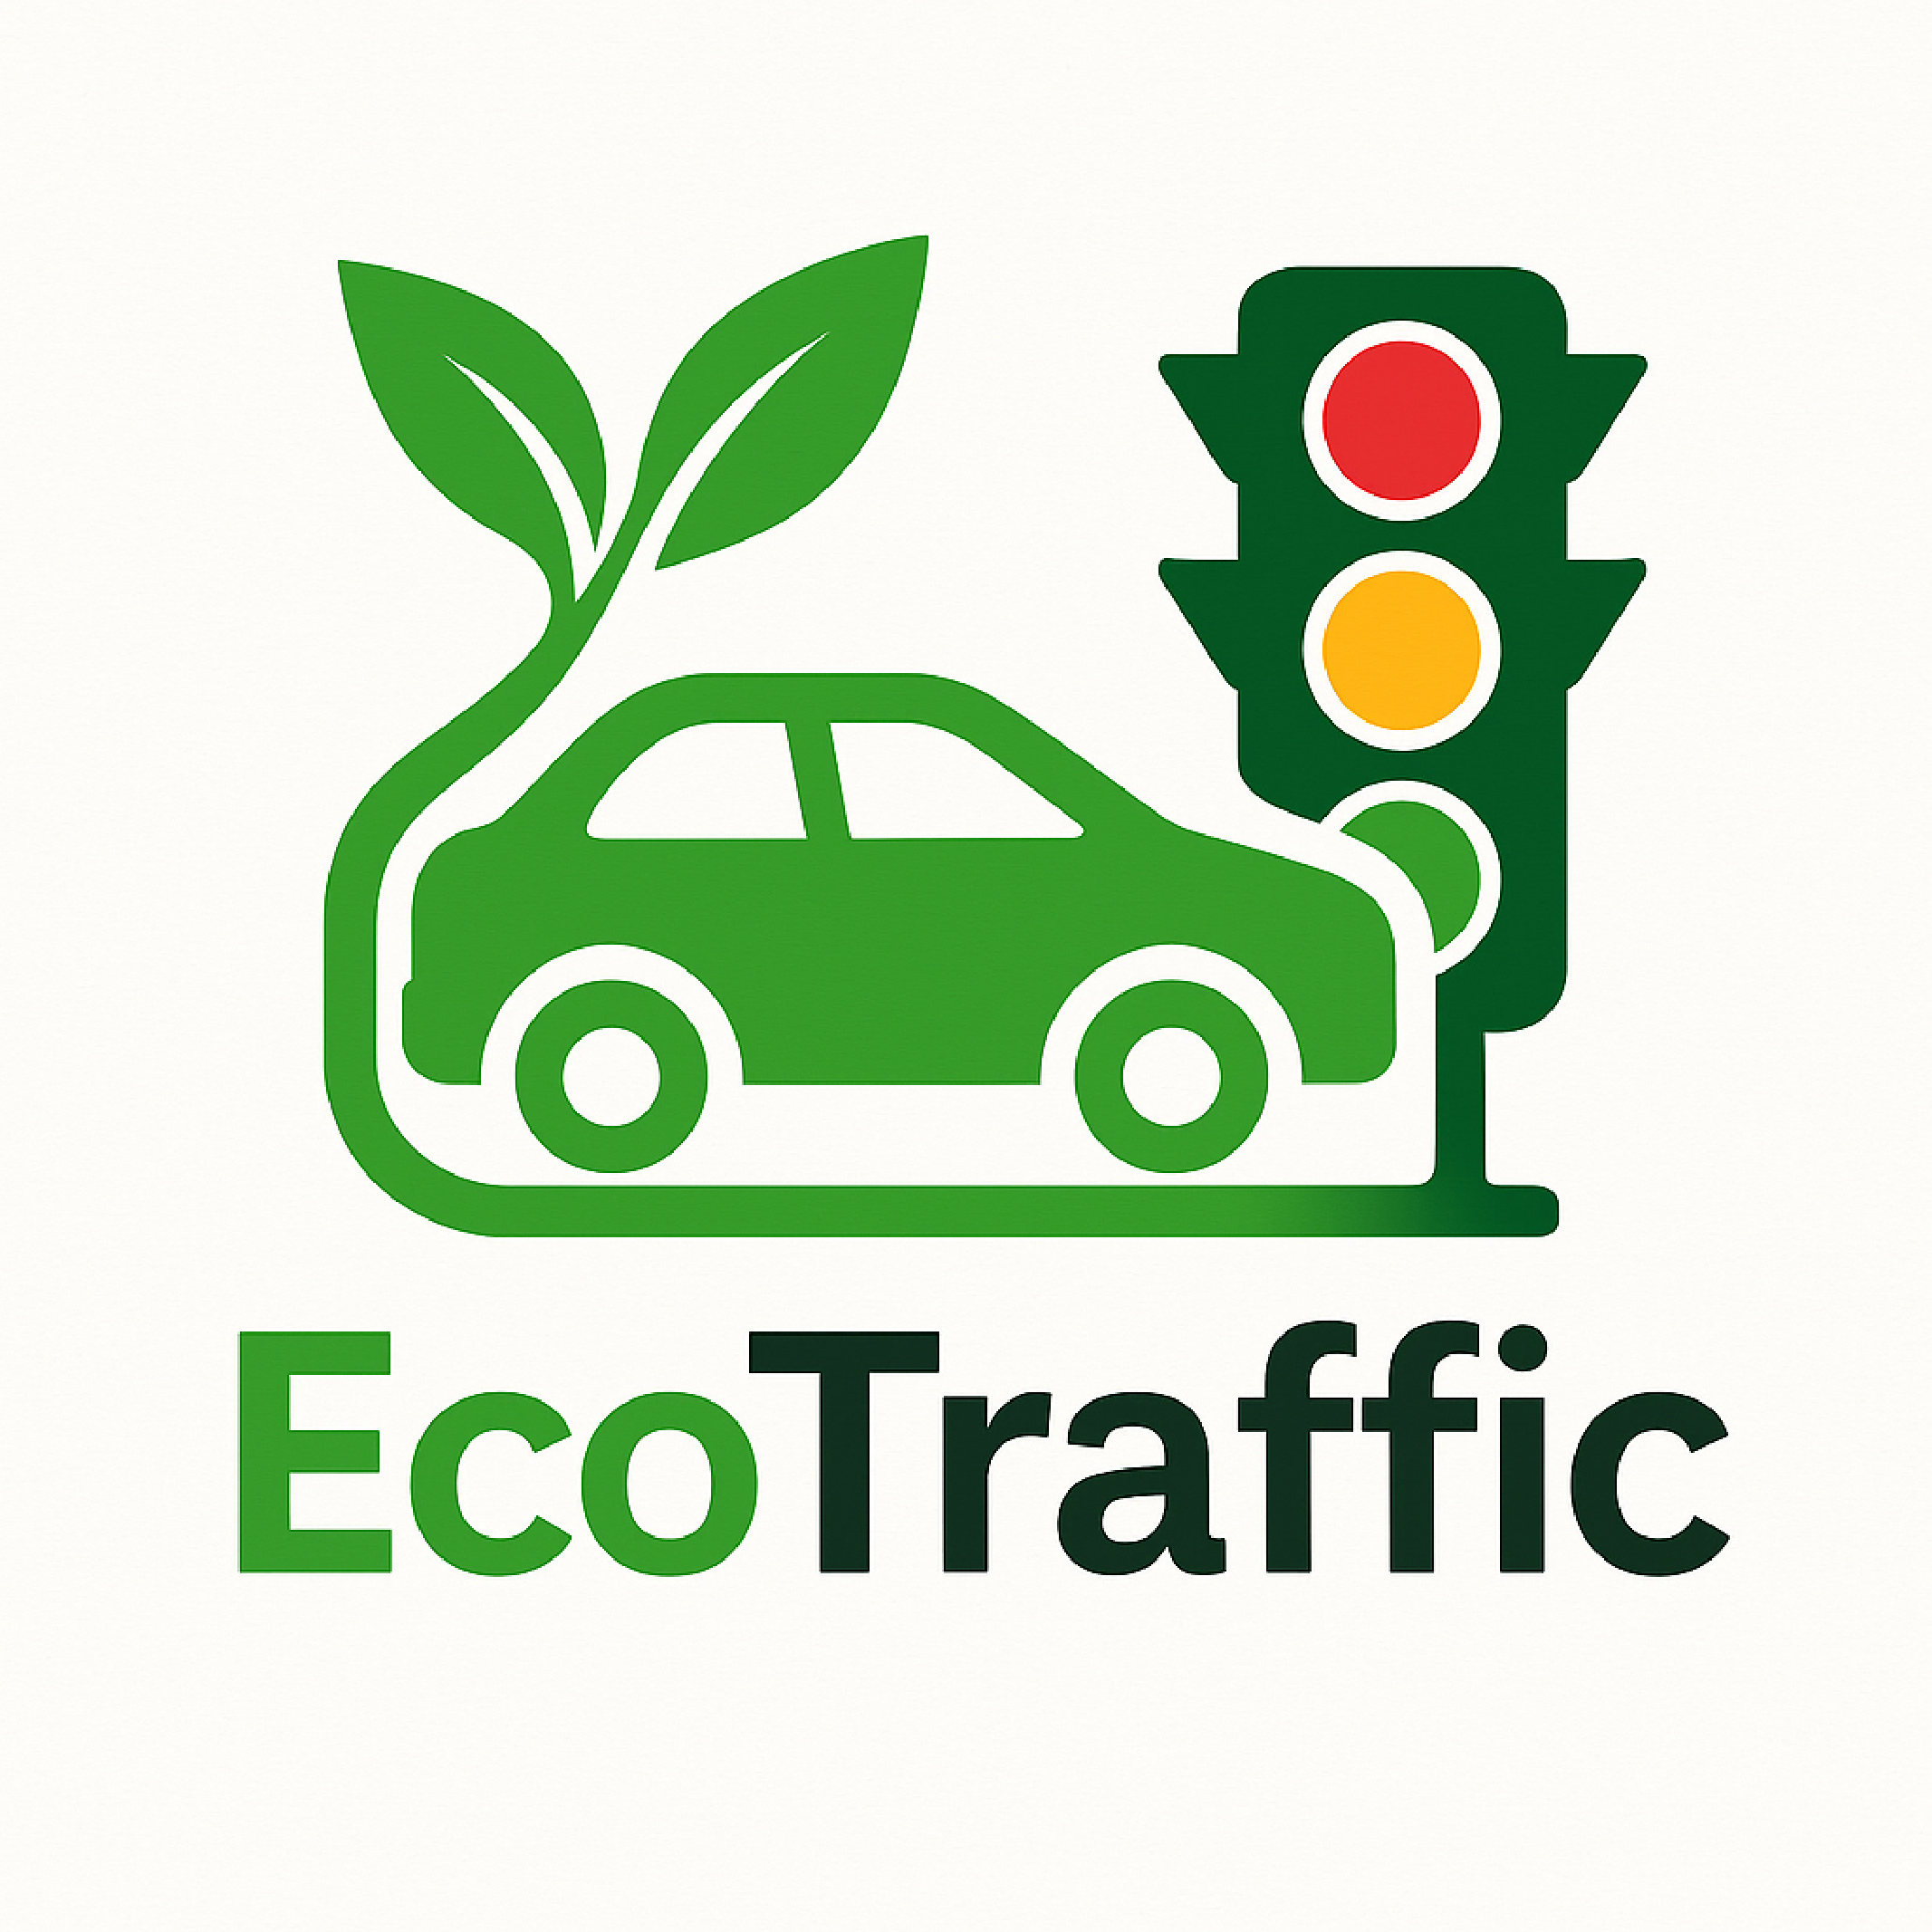
\includegraphics[scale=0.25]{images/EcoTraffic_logo.pdf}  
    \maketitle
    Version 1.0.0
  \end{center}  
\end{textblock*}


\blankpage

% ============== Indice ============== %
\pagenumbering{roman}
\tableofcontents
\afterpage{\blankpage}
\newpage
\pagenumbering{arabic}

\chapter{The Project and the project goals}
\section{The problem}
Two urgent global concerns are environmental sustainability and climate
change; because of air pollution and greenhouse gas emissions,
transportation, especially urban commuting, contributes to worsening
those issues.
\section{The goal}

We want to dynamically modify the duration of traffic lights on the main
roads in the city depending on the directions from where we observe the
main traffic movements. For instance, if, at a certain point in time, we
observe that the traffic flow on a certain road A is significantly
higher than in the crossing roads, then we may decide to extend, for
instance, for one hour, the duration of green lights on A (and,
consequently, extend the duration of red lights in the crossing
roads).\\
We want to analyze the daily traffic patterns and identify possible
optimizations in terms of one-way roads, traffic lights configuration,
and public transport schedule.\\
We want to collect information about the planning of events attracting
large crowds (e.g., important sport events, concerts, fairs) and define
event-specific configurations for traffic lights, roads and public
transport schedules.

\section{Stakeholders}
\begin{itemize}
  \item Drivers: benefit from reduced waiting times and improved traffic flow.
  \item Citizens: benefit from lower air pollution and enhanced public transport.
  \item Urban Area Managers: responsible for optimizing city mobility and approving changes.
  \item Event Planners: coordinate with the system for efficient management of large events.
\end{itemize}

\subsection{Non-Human Actors}
\begin{itemize}
  \item Traffic Lights: get its state set from the EcoTraffic system for a determined period.
  \item Sensor Infrastructure: send sensor information to the EcoTraffic system via data bus.
  \item Public Transport Microservice: sends public transport schedules to the EcoTraffic system via function calls.
  \item News Channel: transmits information about city events to the EcoTraffic system.
\end{itemize}

\section{Use Cases}\label{sec:use-cases}
\subsection{Scenarios (to modify)}\label{subsec:scenarios}

\subsubsection{Traffic light duration adjustment}\label{subsubsec:traffic-light-duration}

\begin{enumerate}
\item
  During peak traffic hours, vehicles take more than necessary to cross a
  particular intersection coming from a busy road, while the crossing
  road is less used.
\item
  The traffic system sensor measures crossing times and publishes them on the
  message bus.
\item
  EcoTraffic retrieves and stores the data in a database.
\item
  EcoTraffic analyzes the crossing times to detect imbalances in traffic flow.
\item
  If an imbalance is detected, EcoTraffic computes adjusted green light durations for the affected intersections.
\item
  EcoTraffic sends the updated timings to the traffic light control system.
\item
  EcoTraffic records the modifications performed in a log file.
\end{enumerate}

\subsubsection{Daily Analysis and optimization}\label{subsubsec:daily-analysis}

\begin{enumerate}
\item
  At 00:10 AM, EcoTraffic retrieve daily data from the
  database.
\item
  EcoTraffic analyzes this data to detect daily traffic patterns and to
  find possible optimization in terms of one-way roads, traffic light
  configuration, and public transport schedules.
\item
  EcoTraffic retrieves the current transport schedules via the public transport microservice.
\item
  Suggested changes are stored in the database for review by the Urban Area Manager (UAM).
\item
  Once the UAM accesses the system, suggestions are displayed for approval or rejection.
\item
  EcoTraffic records the Urban Area Manager's decision in a log file for yearly reporting.
\item
  EcoTraffic sends the accepted suggestions to the traffic light control system.
\end{enumerate}

\subsubsection{Traffic Zone Optimization}\label{subsubsec:traffic-zone}

\begin{enumerate}
\item
  The Urban Area Manager asks to EcoTraffic to verify if a certain zone
  is optimized in terms of one-way roads, traffic lights configuration,
  and public transport schedule.
\item
  EcoTraffic retrieves the traffic patterns of the
  zone from the database.
\item
  EcoTraffic analyzes the data suggest improvements to one-way roads and traffic light configuration.
\item
  EcoTraffic retrieves the current transport schedules via the public transport microservice
  to get all the bus lines that have a stop
  into the area to optimize.
\item
  Using this data, EcoTraffic proposes an optimized configuration. (i.e.
  if in the zone there's a school, then the system could anticipate the
  timetable of the stops near that to avoid the students arriving late
  or could suggest increasing the number of buses in the area).
\item
  EcoTraffic presents to the UAM the recommendations and waits till the
  UAM decides to accept or reject the recommendation and stores the
  decision.
\item
  EcoTraffic records the Urban Area Manager's decision in a log file for yearly reporting.
\item
  EcoTraffic sends the accepted suggestions to the traffic light control system.
\end{enumerate}

\subsubsection{Event-specific configurations}\label{subsubsec:event-specific}

\begin{enumerate}
\item
  News channel publishes information about upcoming events with the
  expected attendance.
\item
  EcoTraffic receives event information from the news channel, categorizes it by expected attendance, location, and scheduled time.
\item
  EcoTraffic analyzes historical traffic patterns from similar events.
\item
  EcoTraffic retrieves public transport schedules.
\item
  EcoTraffic generates event-specific configuration recommendations for
  traffic lights and roads.
\item
  The UAM accesses to EcoTraffic and reviews the suggestions proposed
  and decides to accept or reject them.
\item
  EcoTraffic records the Urban Area Manager's decision in a log file for yearly reporting.
\item
  EcoTraffic sends the accepted suggestions to the traffic light control system.
\end{enumerate}

\subsubsection{Citizen views public traffic reports}\label{subsubsec:citizen-views}

\begin{enumerate}
\item
  A citizen accesses the EcoTraffic public portal and selects either daily or yearly traffic reports.

  \begin{enumerate}
  \item
  The citizen selects "Daily Traffic Reports" and chooses the date and
    time.
    \begin{enumerate}
    \item
      EcoTraffic retrieves daily report data from the database service.
    \item
      EcoTraffic displays report showing:

  \begin{enumerate}
        \def\labelenumiv{\alph{enumiv}.}
        \item
          Average traffic flow on main roads.
        \item
          Visualization of peak congestion periods.
        \item
          List of actions taken automatically.
        \item
          Traffic prediction for tomorrow.
        \end{enumerate}
      \end{enumerate}
    \item
    The citizen selects the "Yearly Reports" option.
  
      \begin{enumerate}
      \item
        EcoTraffic displays yearly report options.
      \item
        EcoTraffic retrieves yearly report data from the database service.
      \item
        EcoTraffic displays a comprehensive report showing:
  
        \begin{enumerate}
        \def\labelenumiv{\alph{enumiv}.}
        \item
          Suggested actions that were accepted.
        \item
          Suggested actions that were rejected.
        \end{enumerate}
      \end{enumerate}
    \end{enumerate}
  \end{enumerate}

\subsubsection{UAM views optimization to approve or reject}\label{subsubsec:uam-views}

\begin{enumerate}
\item
  UAM access to EcoTraffic public portal.
\item
  EcoTraffic presents the list of pending optimization suggestions awaiting UAM approval or rejection.
\item
  The UAM analyzes each suggestion and decide to approve or reject
  choosing an option displayed.
\item
  EcoTraffic records the UAM's decision in a log file for yearly reporting.
\end{enumerate}

\subsection{Use case diagrams (to modify and insert diagrams)}
\subsubsection{Traffic light duration adjustment}

\rowcolors{3}{gray!10}{white}

\begin{longtable}{>{\raggedright\arraybackslash}p{0.45\textwidth} >{\raggedright\arraybackslash}p{0.45\textwidth}}
\toprule
\textbf{Aspect} & \textbf{Description} \\
\midrule
\endhead
\midrule
\multicolumn{2}{r}{\textit{Continues on next page}} \\
\endfoot
\bottomrule
\endlastfoot

Actors & Sensors, Traffic lights, Database \\
Entry condition & After sensors measure new crossing times, new data arrives on the bus. \\
Flow of events &
\begin{enumerate}
  \item EcoTraffic reads data from the message bus.
  \item EcoTraffic saves the received data to the database.
  \item EcoTraffic compares the crossing times of the roads in the crossings.
  \item If EcoTraffic detects traffic load imbalance, the system computes the green light duration to optimize vehicle flow in the more congested direction.
\end{enumerate}
\\
Exit condition & The system sends the adjusted times to the traffic lights control system. \\
\end{longtable}


\subsubsection{Daily Analysis and Optimization}

\rowcolors{3}{gray!10}{white}
\begin{longtable}{>{\raggedright\arraybackslash}p{0.45\textwidth} >{\raggedright\arraybackslash}p{0.45\textwidth}}
\toprule
\textbf{Aspect} & \textbf{Description} \\
\midrule
\endhead
\midrule
\multicolumn{2}{r}{\textit{Continues on next page}} \\
\endfoot
\bottomrule
\endlastfoot

Actors & Webservice, Database \\
Entry condition & It's ten past midnight. \\
Flow of events &
\begin{enumerate}
  \item EcoTraffic queries the database to get all the crossing times measured the day before.
  \item EcoTraffic analyzes the data retrieved to obtain traffic patterns.
  \item EcoTraffic analyzes the traffic patterns to identify potential optimizations regarding one-way roads and traffic light configurations.
  \item EcoTraffic retrieves public transport schedules via microservice using getScheduleByStreet and getScheduleByLine operations.
  \item EcoTraffic tries to find better schedules for the public transport line.
\end{enumerate}
\\
Exit condition & The system writes into the database the possible optimization found. \\
\end{longtable}

\subsubsection{Traffic zone optimization}

\rowcolors{3}{gray!10}{white}
\begin{longtable}{>{\raggedright\arraybackslash}p{0.45\textwidth} >{\raggedright\arraybackslash}p{0.45\textwidth}}
\toprule
\textbf{Aspect} & \textbf{Description} \\
\midrule
\endhead
\midrule
\multicolumn{2}{r}{\textit{Continues on next page}} \\
\endfoot
\bottomrule
\endlastfoot

Actors & Urban area manager, Public Transport Microservice, Database \\
Entry condition & UAM accesses the EcoTraffic public portal and decides to request optimization of a certain area. \\
Flow of events &
\begin{enumerate}
  \item EcoTraffic queries the database to obtain the crossing times of the zone indicated by the UAM.
  \item EcoTraffic analyzes the data to identify potential optimizations regarding one-way roads and traffic light configurations.
  \item EcoTraffic retrieves public transport schedules via microservice using getScheduleByStreet and getScheduleByLine operations.
  \item EcoTraffic tries to find better schedules for the public transport line.
  \item The system sends the new scheduling and configuration proposal to the UAM for approval.
  \item The system waits for the answer.
  \item When the decision is taken, the answer is written into a log file.
  \item If the decision is to accept the proposal, EcoTraffic sends the new configuration to the traffic light control system.
\end{enumerate}
\\
Exit condition & Successful write of the log and successful communication with the traffic light control system. \\
\end{longtable}

\subsubsection{Event-specific configurations}

\rowcolors{3}{gray!10}{white}
\begin{longtable}{>{\raggedright\arraybackslash}p{0.45\textwidth} >{\raggedright\arraybackslash}p{0.45\textwidth}}
\toprule
\textbf{Aspect} & \textbf{Description} \\
\midrule
\endhead
\midrule
\multicolumn{2}{r}{\textit{Continues on next page}} \\
\endfoot
\bottomrule
\endlastfoot

Actors & News channel, UAM, Public Transport Microservice \\
Entry condition & News channel publishes information about upcoming events. \\
Flow of events &
\begin{enumerate}
  \item EcoTraffic categorizes the scale of the event by attendance.
  \item EcoTraffic queries the database for historical traffic patterns and reviews past decisions recorded in log files for similar events.
  \item EcoTraffic retrieves public transport schedules via microservice using getScheduleByStreet and getScheduleByLine operations.
  \item Using the collected data, EcoTraffic generates event-specific configurations that are optimized in terms of one-way roads, traffic light configurations, public transport schedules.
\end{enumerate}
\\
Exit condition & The system writes into the database the possible optimization found. \\
\end{longtable}

\subsubsection{Citizen views public traffic reports}

\rowcolors{3}{gray!10}{white}
\begin{longtable}{>{\raggedright\arraybackslash}p{0.45\textwidth} >{\raggedright\arraybackslash}p{0.45\textwidth}}
\toprule
\textbf{Aspect} & \textbf{Description} \\
\midrule
\endhead
\midrule
\multicolumn{2}{r}{\textit{Continues on next page}} \\
\endfoot
\bottomrule
\endlastfoot

Actors & Citizen \\
Entry condition & Citizen accesses EcoTraffic public portal. \\
Flow of events &
\begin{enumerate}
  \item The system presents options for viewing reports.
  \item The citizen selects the type of information that they want to be displayed.
  \item The system retrieves daily or yearly data from the database service.
  \item The system elaborates the data to facilitate interpretation.
  \item The system displays a report with the elaborated data.
  \item The citizen chooses between seeing more information or exiting the portal.
\end{enumerate}
\\
Exit condition & The citizen exits the portal. \\
\end{longtable}

\subsubsection{UAM views optimization to approve or reject}

\rowcolors{3}{gray!10}{white}
\begin{longtable}{>{\raggedright\arraybackslash}p{0.45\textwidth} >{\raggedright\arraybackslash}p{0.45\textwidth}}
\toprule
\textbf{Aspect} & \textbf{Description} \\
\midrule
\endhead
\midrule
\multicolumn{2}{r}{\textit{Continues on next page}} \\
\endfoot
\bottomrule
\endlastfoot

Actors & UAM \\
Entry condition & UAM accesses the EcoTraffic public portal and decides to view the optimization waiting for approval. \\
Flow of events &
\begin{enumerate}
  \item EcoTraffic queries the database for the optimization proposals waiting for approval.
  \item EcoTraffic elaborates on the data to facilitate interpretation.
  \item EcoTraffic displays all the decisions to be taken.
  \item EcoTraffic waits for the UAM to answer to each request.
  \item Every time a decision is taken EcoTraffic stores it into a log file.
  \item If the decision is to accept the proposal, EcoTraffic sends the new configuration to the traffic light control system.
\end{enumerate}
\\
Exit condition & All the decisions have been taken. \\
\end{longtable}

\section{Domain assumption}
\begin{domain_assumption}
\item
  The sensor infrastructure works correctly and at low latency 24/7.
\item
  The traffic lights are not faulty and set their state correctly in
  time from the EcoTraffic system.
\item
  Drivers behave according to the traffic light state.
\item
  No car can obstruct the passage in the crossing no matter the reason.
\item
  Events planners always report to the news channel up-to-date events in
  the city.
\item
  The public transport microservice always returns the right timetable
  given a line or the name of a street.
\item
  The public transport microservice, the sensor infrastructure, the database and the traffic light control system 
  are always available and responds in a timely manner.
\item
  The traffic light control system is able to schedule future adjustments in the traffic light state.

\end{domain_assumption}
\section{Requirements}
\subsection{Functional Requirements}

\begin{functional_requirements}
\item
  In any circumstance, the system must not allow two orthogonal traffic
  lights to be green at the same time.
\item
  The system must modify the duration of the green lights to reduce
  traffic.
\item
  The system shall process and aggregate traffic data to identify
  traffic flow patterns.
\item
  The system should send adjustment commands to the traffic light
  control system.
\item
  The system should be able to write to a log file what is needed.
\item
  The system shall generate optimization suggestions for one-way road
  and traffic light configurations.
\item
  The system shall generate optimization suggestions for public
  transport schedules.
\item
  The system shall continuously receive data from both the message bus
  and the news channel.
\item
  The system must gather data from the microservice.
\item
  The system must assess the potential traffic impact of planned events.
\item
  The system shall generate event-specific suggestions for public
  transport adjustments.
\item
  The system shall present suggestions to urban area managers for
  review.
\item
  The system shall record and apply the acceptance or rejection of the
  proposal by the urban area managers.
\item
  The system shall generate daily reports on average traffic flow.
\item
  The system shall generate yearly reports on suggestions proposed and
  their outcome.
\item
  The system shall publish reports for public access.
\end{functional_requirements}

\subsection{Non-Functional Requirements}

\begin{non_functional_requirements}
\item
  The system shall process sensor data in real-time.
\item
  The system should be available 24/7.
\item
  The system shall implement traffic light adjustments in 15 seconds.
\item
  The system shall generate reports within 1 hour after midnight.
\item
  The system should maintain data consistency during communication with
  external systems.
\item
  The system should be scalable to support the addition of new sensors and bus lines 
  without requiring significant changes to the architecture.
\end{non_functional_requirements}

\subsection{Constraints (to modify, insert something to use the
external services)}

\begin{constraints}
\item
  The setLight function must be atomical.
\item
  The call to the microservice must be done using an API REST.
\end{constraints}

\chapter{Design}

\section{Architecture}
\subsection{Components diagram}

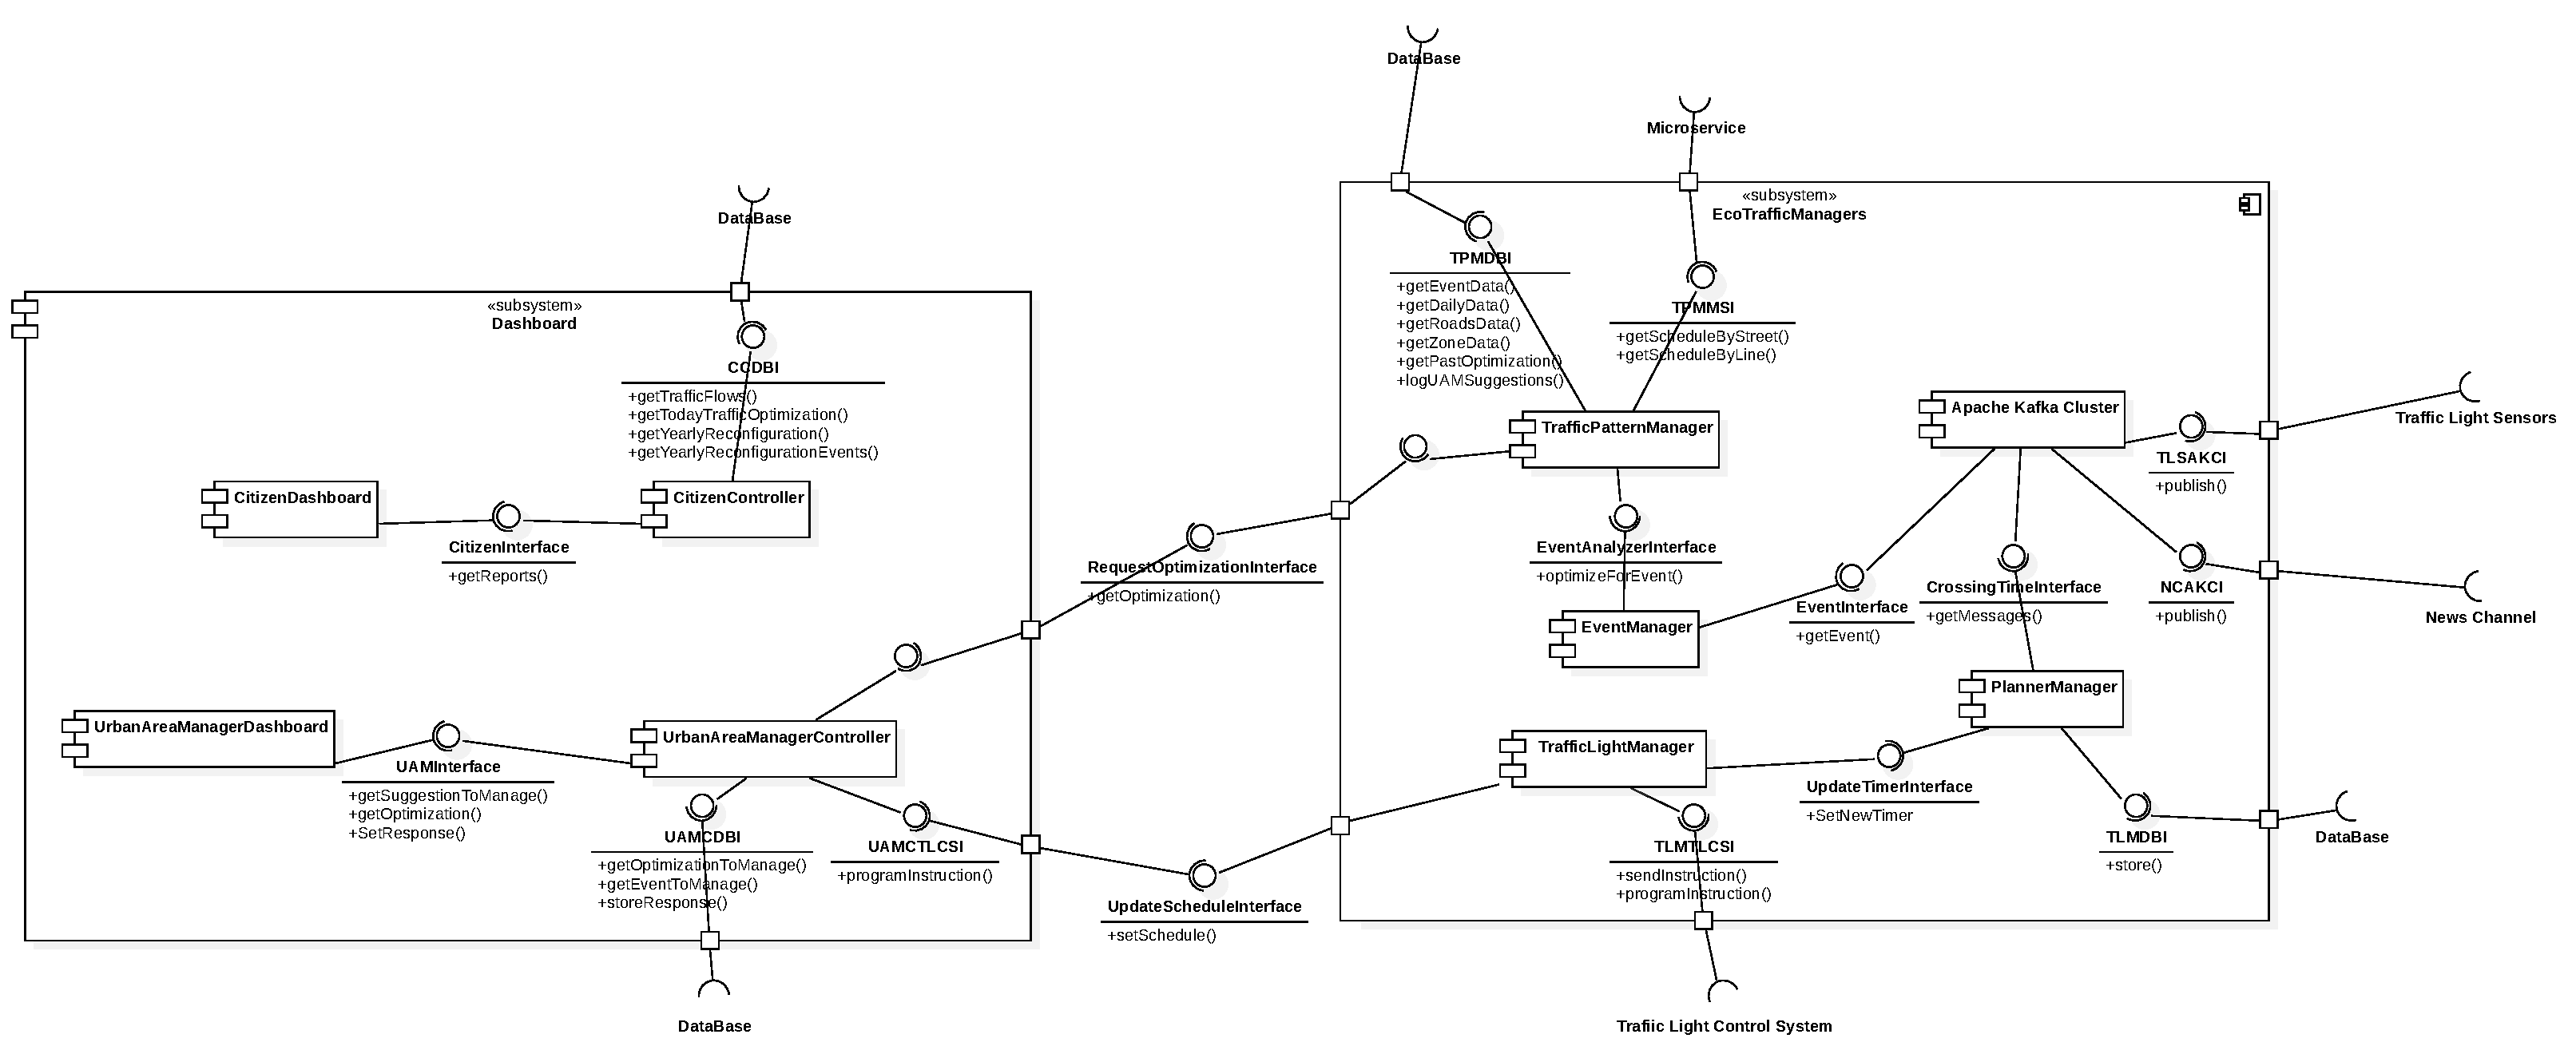
\includegraphics[width=\linewidth]{images/svg/ComponentDiagram.pdf}
There have been inserted multiple interfaces named "Database" for readability. Actually, there is only one database that is used by all the components.
Its structure is shown in the next diagram:\\
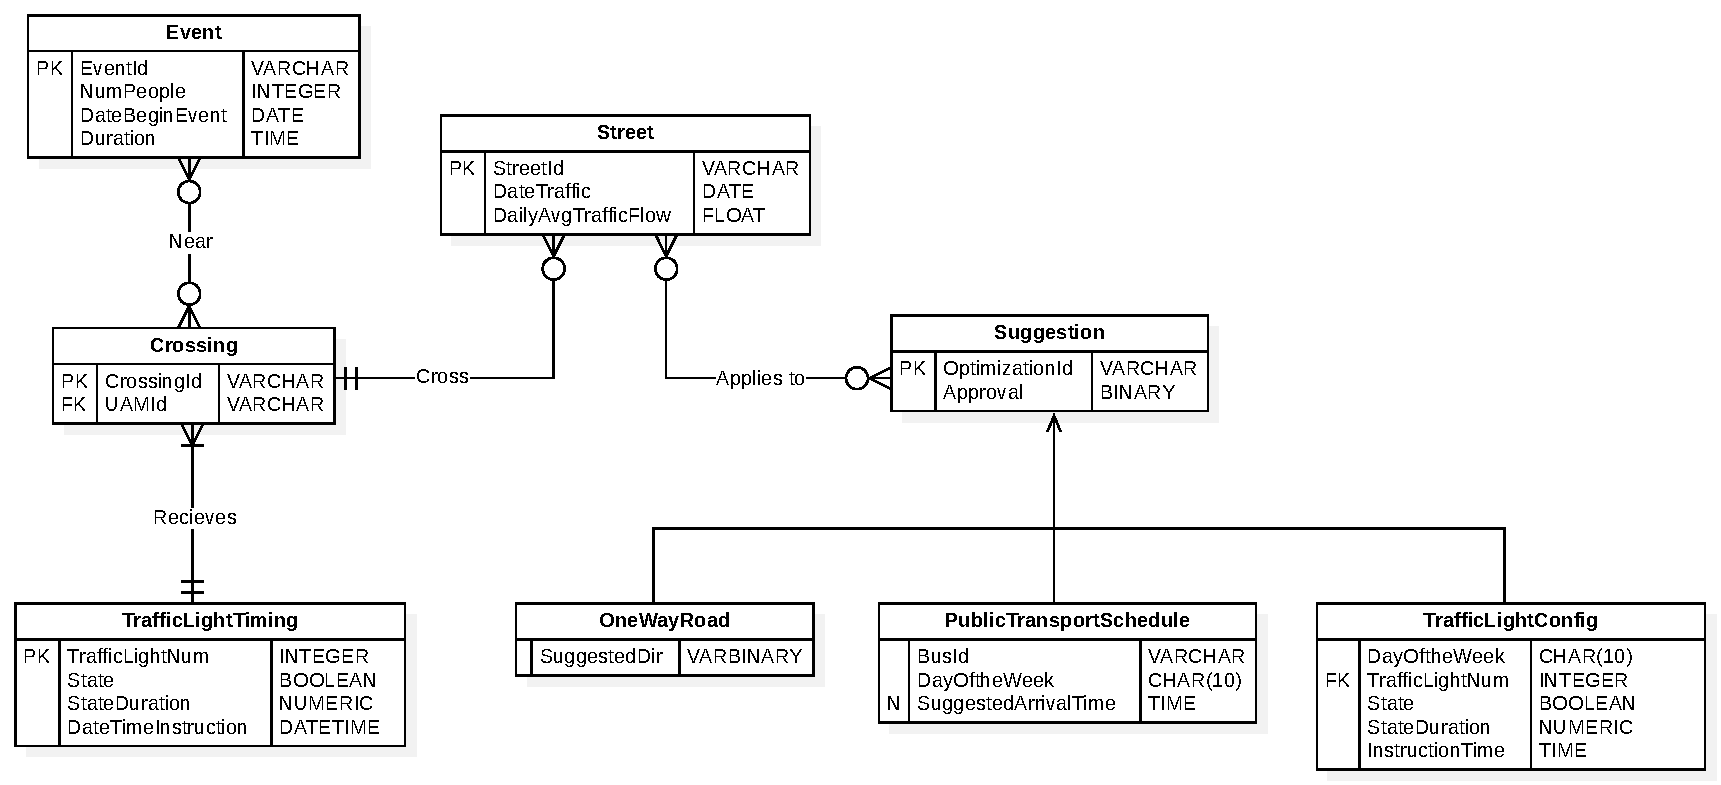
\includegraphics[width=\linewidth]{images/svg/DiagrammaER_V2.pdf}

\subsection{Subsystems and components}

The EcoTrafficManagers subsystem includes the following components:


\begin{itemize}
\item
  \textbf{ApacheKafkaCluster:} the component is based on a framework for
  the event-driven paradigm and it includes primitives to create event
  producers and consumers and a runtime infrastructure to handle event
  transfer. This component it's the one responsible for receiving the data
  from the sensors system and from the news channel and to distribute
  them to the right components, which will then process and analyze them.
  More information can be found at \url{https://kafka.apache.org/}.
\item
  \textbf{TrafficLightManager:} this component receives the data
  measured by the sensors system from the ApacheKafkaCluster and
  provides a method to analyze this data to find unbalanced traffic loads
  into a crossing, to compute the new time in which the green light is
  switched on to reduce traffic congestion, to store into the database
  of the system the data obtained from the ApacheKafkaCluster and to
  connect to the control system of the traffic lights to apply the right
  modifications.
\item
  \textbf{EventManager:} this component receives the event specification
  from the ApacheKafkaCluster after that the news channel has published
  them. This component provides methods to retrieve information (such
  as the event type, the date, the place and the expected attendance)
  and a method to call the TrafficPatternManager component to optimize
  the event configuration to reduce traffic load.
\item
  \textbf{TrafficPatternManager:} this component could be called by
  three events. The first is when the EventManager calls it to perform
  event-based optimization, in this case, the component queries the
  database to find similar events and the daily traffic patterns in the
  zone where the event takes place, then generate possible optimizations
  from this data and from the timetables obtained after the
  getScheduleByStreet() and the getScheduleByLine() calls to the
  microservice. The second is when the UrbanAreaManagerController asks
  for an optimization around a specific zone, in this case, the component
  queries the daily traffic patterns in the zone and the timetables and
  tries to optimize the traffic loads. The third takes place
  automatically ten minutes after midnight, in this case, the
  component queries the daily crossing time in all the crossings of the
  area and finds traffic patterns, after that, it tries to optimize in
  terms of one-way roads, traffic lights configuration, and public
  transport schedule.
\end{itemize}

The Dashboard subsystem includes the following components:

\begin{itemize}
\item
  \textbf{CitizenDashboard:} this component shows to the citizen an
  interface from where it can be decided to see the daily reports or the
  yearly ones. After choosing, the component calls the CitizenController
  to get the reports. When the response arrives, the component shows to
  the user the reports.
\item
  \textbf{CitizenController:} this component receives the request from
  the citizen dashboard and then queries the database to satisfy the
  request. After, the data are elaborated and sent to the dashboard.
\item
  \textbf{UrbanAreaManagerDashboard:} this component shows the UAM an
  interface from where it can be decided if to see the pending
  suggestions or to ask the system to optimize all the configurations in
  a specific zone. If the first option is chosen, it calls the
  UrbanAreaManagerController to get the pending suggestions. When the
  response arrives, the component shows to the user the reports and
  waits till all the decisions are taken. When each decision is taken,
  the component sends the answer to the controller. If the second option
  is taken, the dashboard presents the zones in the area and waits for
  the UAM's decision, after it arrives the component sends to the
  controller the requests and waits for the answer, after this arrives
  it displays to the UAM the suggestions, when the decision is taken,
  the component sends the answer to the controller.
\item
  \textbf{UrbanAreaManagerController:} this component is responsible for
  managing the requests arriving from the dashboard and redirecting them
  either to the database if the UAM wants to see the pending suggestions
  or to the TrafficPatternManager if the UAM wants an optimization for a
  specific zone. After the responses arrive, the component sends them to
  the dashboard. If the answer is an optimization the component waits
  for the approval or the rejection and stores the decision.
\end{itemize}
  
\section{Sequence Diagrams}
\subsubsection{Traffic Lights Adjustment}

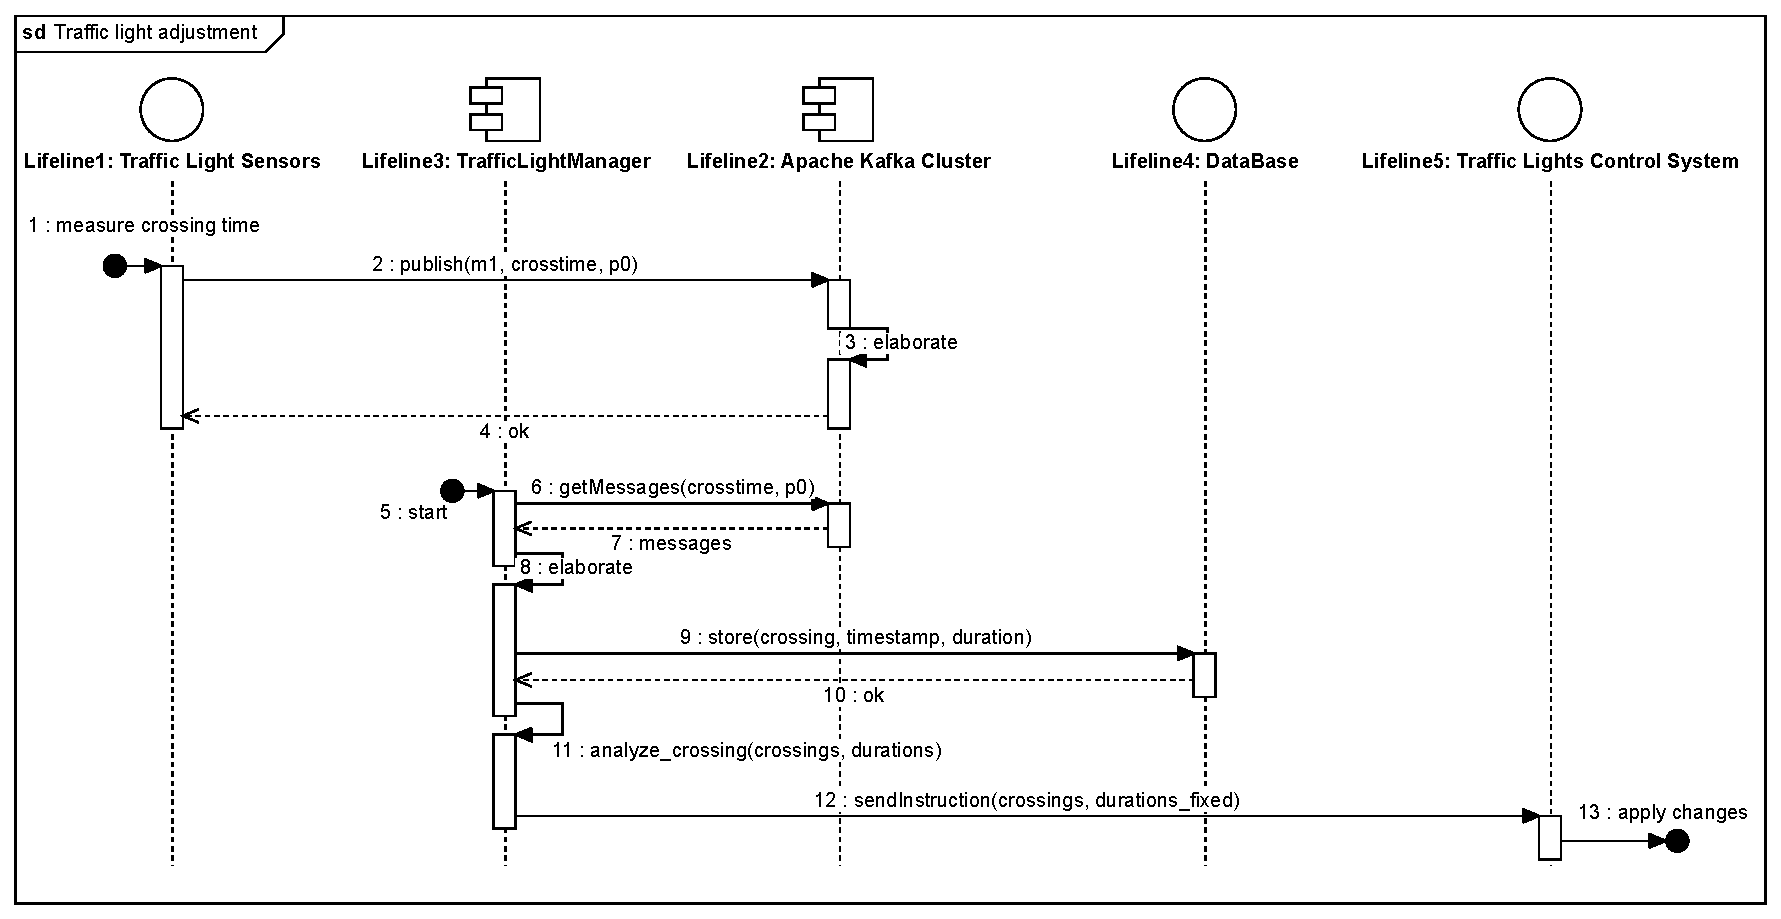
\includegraphics[width=\linewidth]{images/svg/traffic_light_adjustment.pdf}

This sequence diagram shows the communication and data flow involved in
adjusting traffic light timings based on crossing data.

\begin{enumerate}
\item
  The traffic light sensors system measures a crossing time.
\item
  The traffic light sensors system publishes the crossing time on the
  message bus and it's received from the Apache Kafa Cluster.
\item
  The Apache Kafka Cluster performs the operation as shown in this
  diagram.
\item
  The Apache Kafka Cluster responds to the traffic light sensor system.
\item
  TrafficLightManager is working.
\item
  TrafficLightManager tries to get a message.
\item
  The message, if present, is sent to TrafficLightManager. The point 6
  and 7 are better shown in this diagram.
\item
  TrafficLightManager elaborates the message received extracting the
  important information.
\item
  TrafficLightManager sends a message to the database to make it store
  the data received.
\item
  Successful store.
\item
  TrafficLightManager analyzes the data received to find eventually
  unbalanced traffic loads. If it finds them, then it computes also the
  new green light time for a particular traffic light.
\item
  TrafficLightManager sends a message to the traffic light control
  system with the modification to perform.
\item
  Traffic light control system applies the changes
\end{enumerate}


\subsubsection{Traffic Zone Optimization}


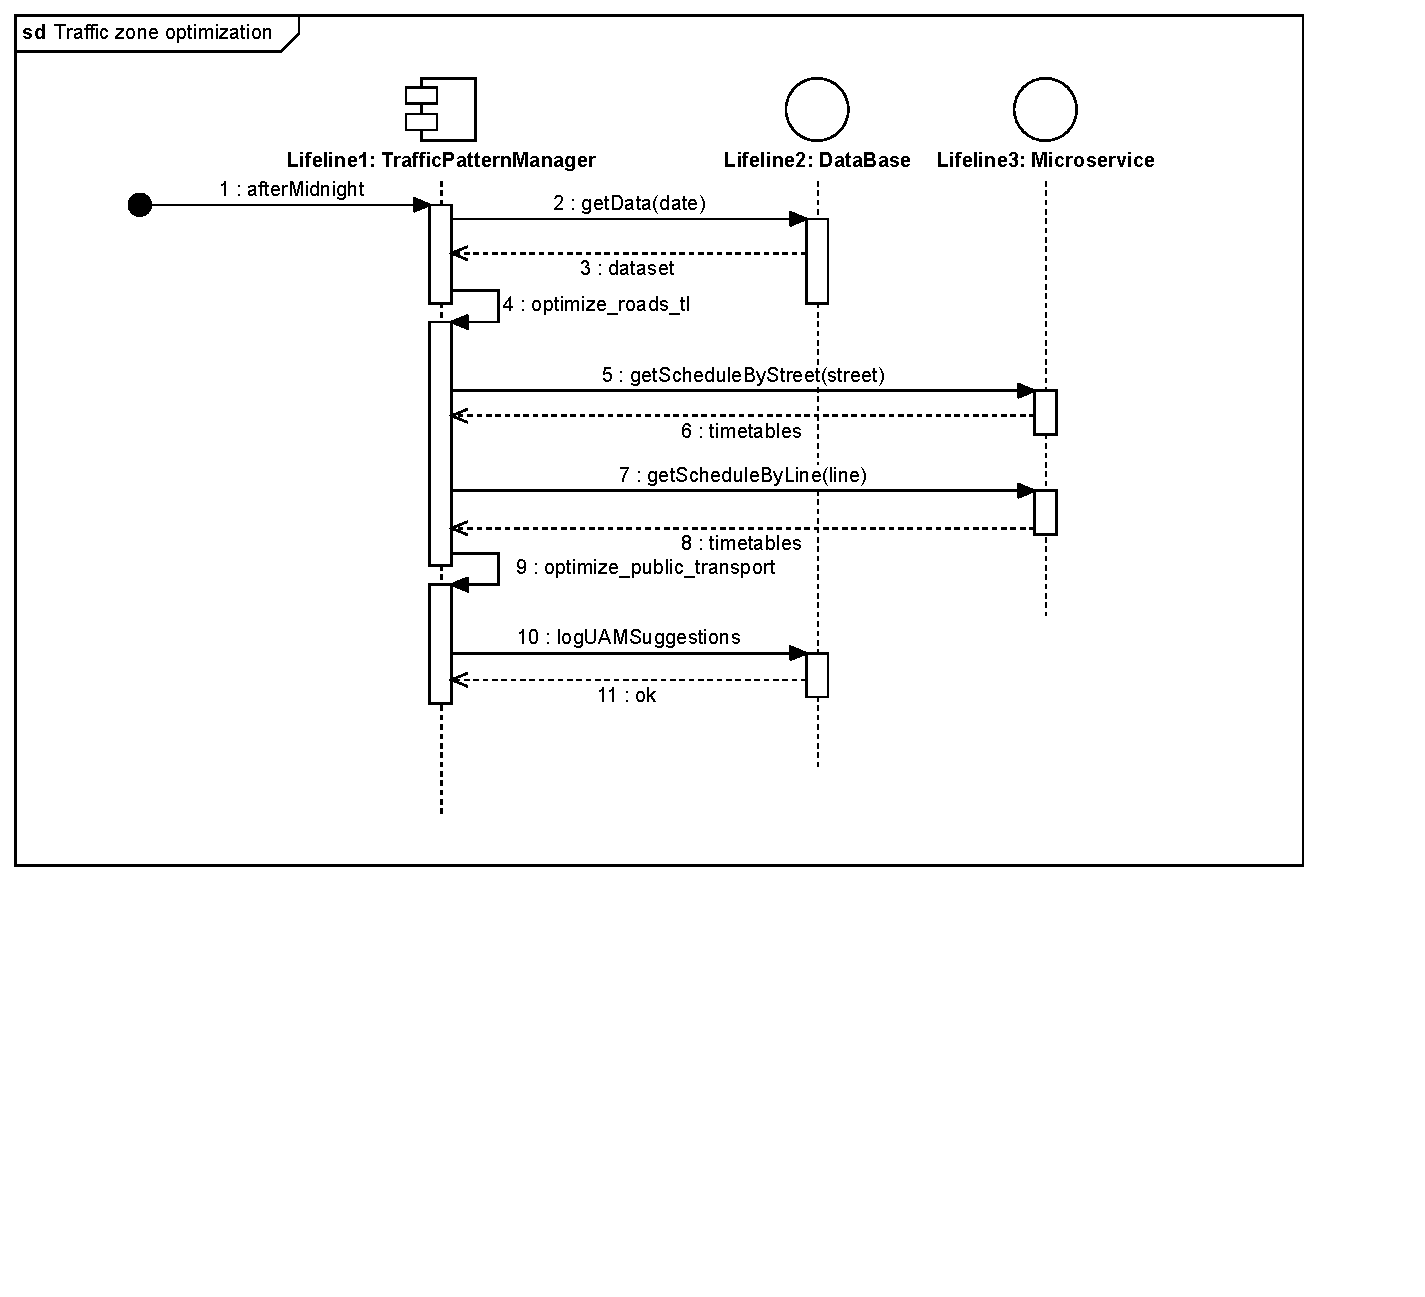
\includegraphics[width=\linewidth]{images/svg/traffic_zone_optimization.pdf}


This sequence diagram illustrates the data flow between TrafficPatternManager, database, and Microservice components for optimizing traffic zones, including both road traffic and public transportation optimization.
\begin{enumerate}
  \item The process starts when the TrafficPatternManager receives an "afterMidnight" trigger or signal.
  \item TrafficPatternManager requests data from the database collected on the date passed as an argument.
  \item The database responds by returning the data to the TrafficPatternManager.
  \item TrafficPatternManager analyzes the data to identify traffic patterns.
  \item TrafficPatternManager stores the patterns in the database.
  \item TrafficPatternManager tries to optimize the road traffic lights to reduce the traffic loads.
  \item	TrafficPatternManager asks for the timetables of the streets to the microsystem provided by the state.
  \item	The microsystem returns the street timetables.
  \item	TrafficPatternManager asks for the timetables of the lines to the microsystem.
  \item	The microsystem returns the line timetables.
  \item TrafficPatternManager tries to optimize public transportation schedules.
  \item TrafficPatternManager logs the suggestions and stores them in the database.
  \item The Microservice responds with an "ok" confirmation message, completing the sequence.
\end{enumerate}

\subsubsection{Event-specific Configuration}


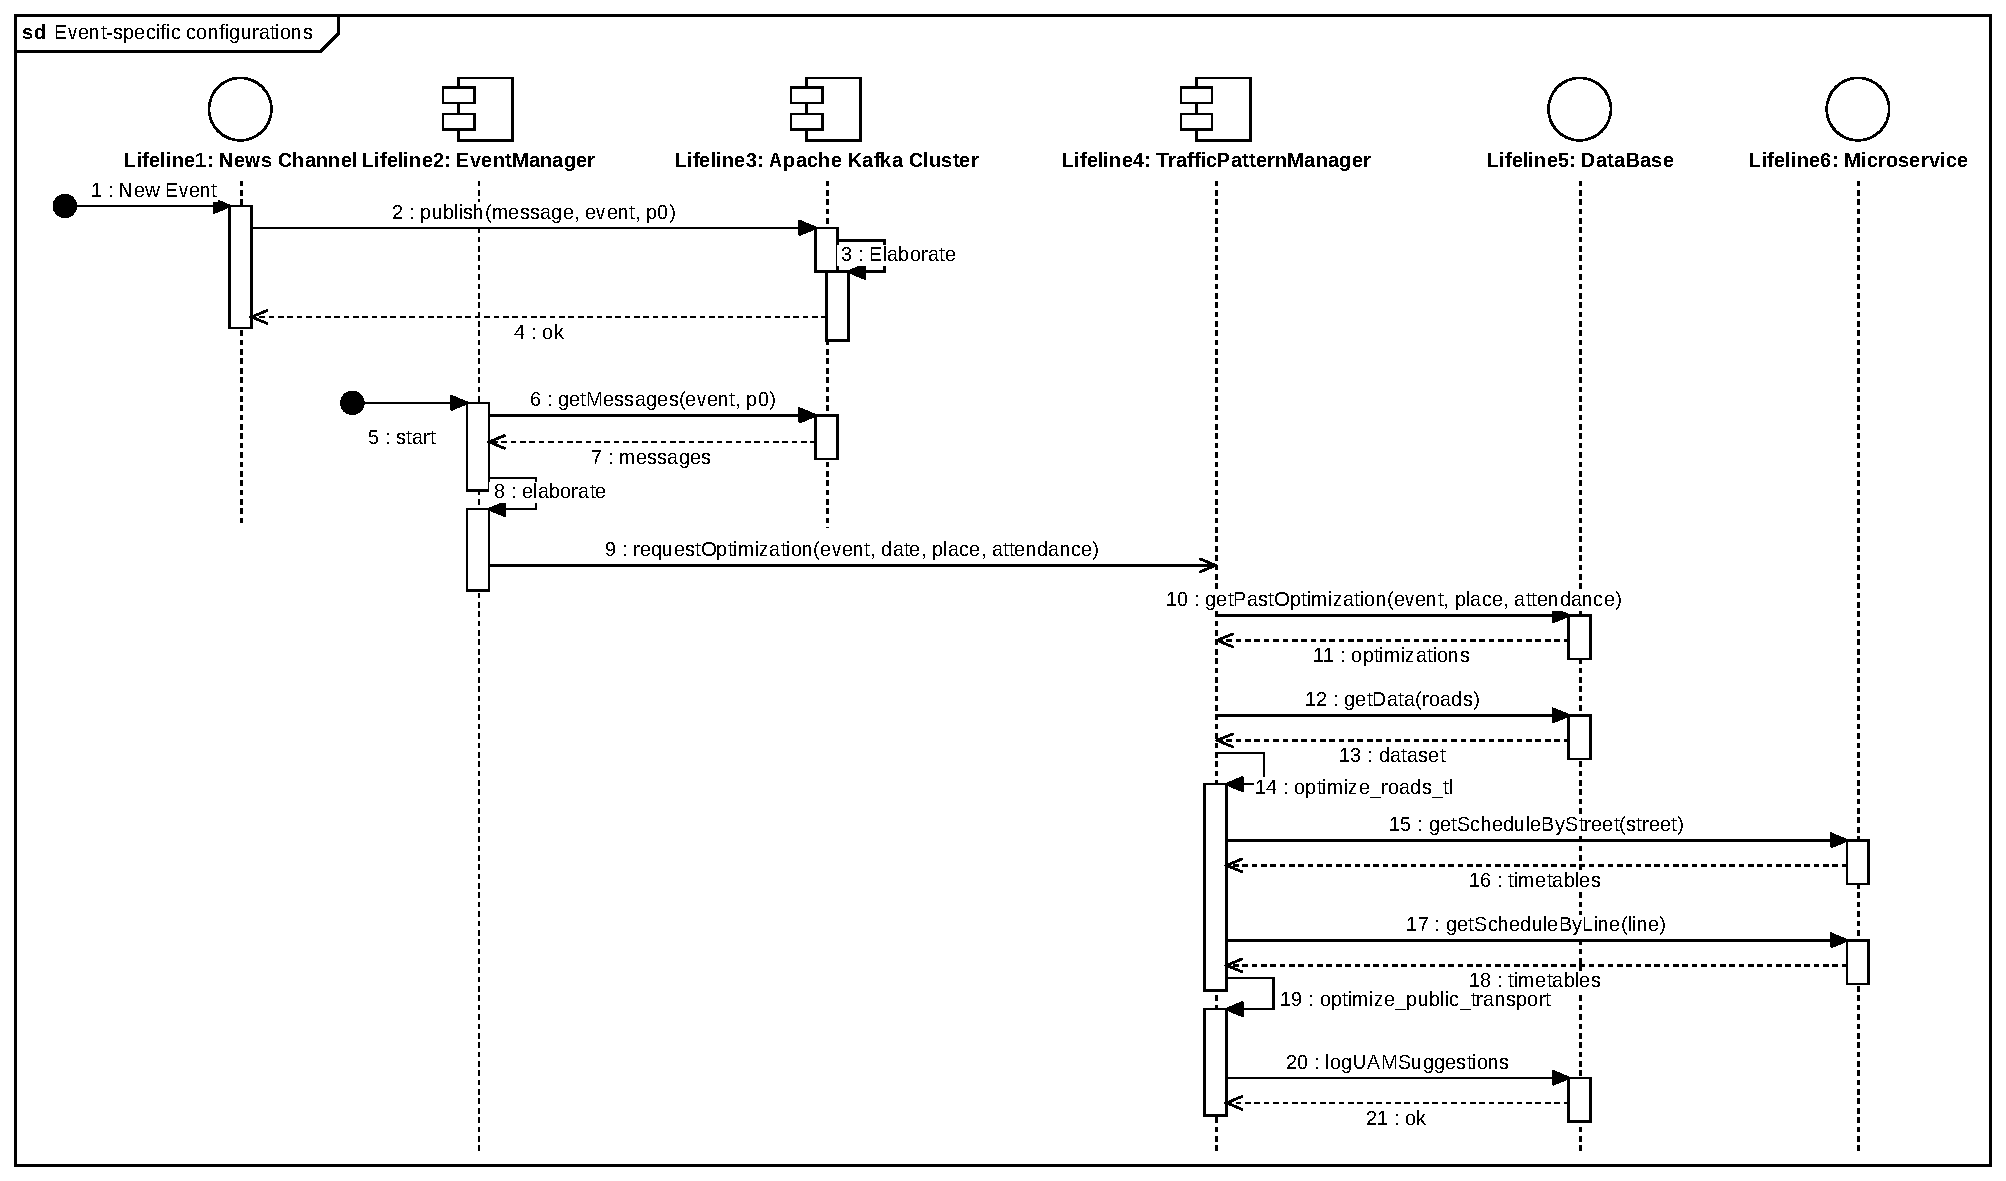
\includegraphics[width=\linewidth]{images/svg/event-specific_configurations.pdf}

This sequence diagram shows the communication and data flow involved in
adjusting traffic light timings based on crossing data.
\begin{enumerate}
  \item Ten minutes past midnight, an automatic process is started in the system and it is managed by the Traffic Pattern Manager.
  \item The Traffic Pattern Manager retrieves data from the database by passing the current date.
  \item	The database then returns a dataset to the Traffic Pattern Manager.
  \item	The Traffic Pattern Manager then optimizes the traffic flow for the whole system of traffic lights.
  \item	Then the Traffic Pattern Manager asks for the timetables of the streets to the microsystem provided by the state.
  \item	The microsystem returns the street timetables.
  \item	The Traffic Pattern Manager asks for the timetables of the lines to the microsystem.
  \item	The microsystem returns the line timetables.
  \item	Then the system proceeds to optimize the public transport tables.
  \item	In the end, the Traffic Pattern Manager logs the suggestions into the database.
  \item	The database returns an ack message in case of successful write.
\end{enumerate}


\subsubsection{Citizen views public reports}


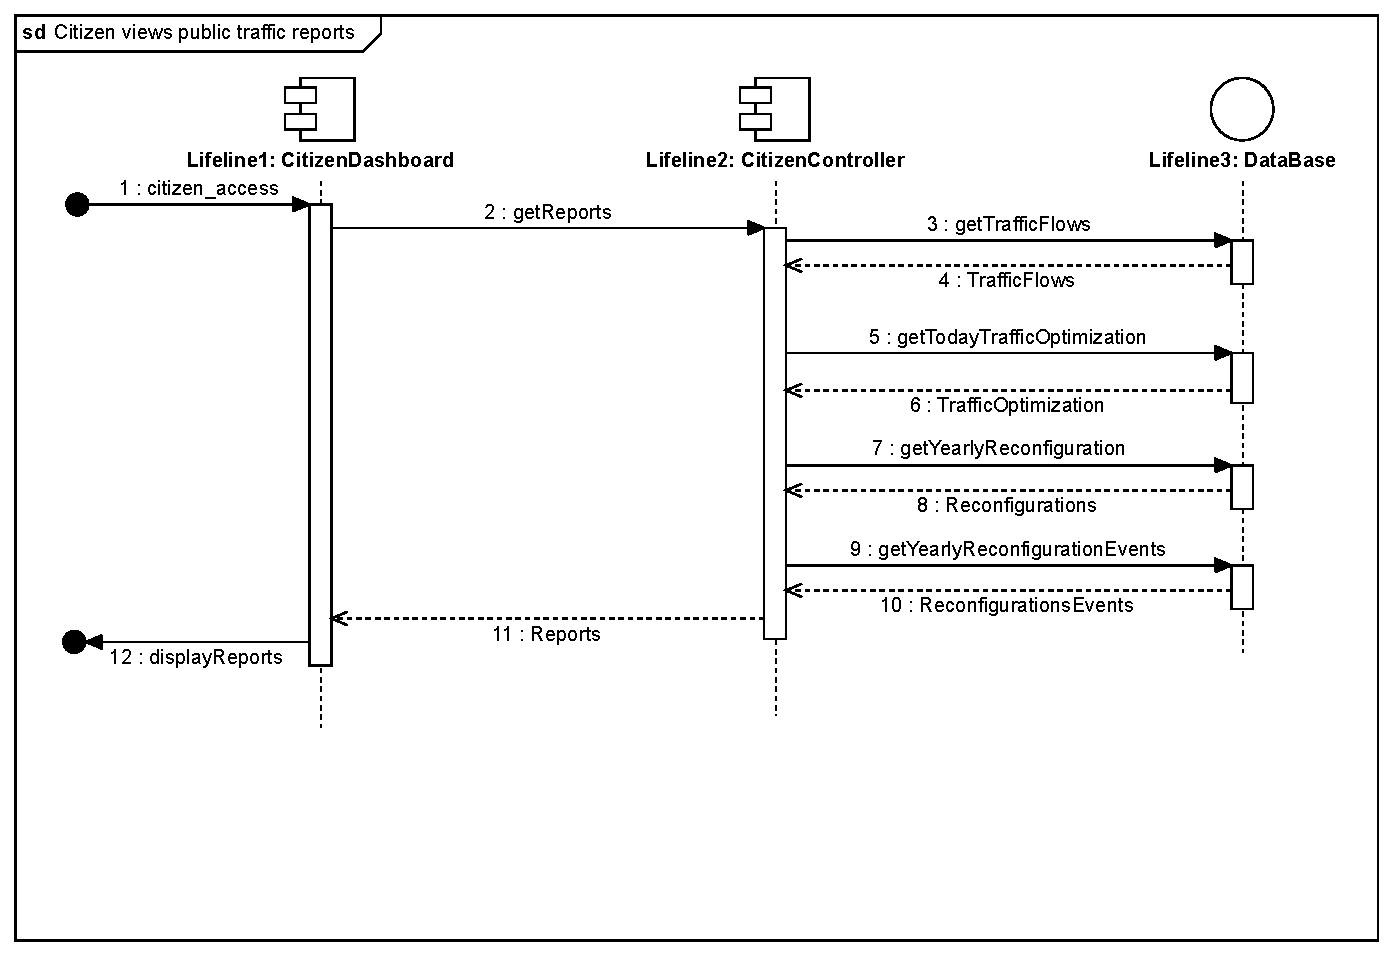
\includegraphics[width=\linewidth]{images/svg/citizen_views_public_traffic_reports.pdf}

This sequence diagram shows the communication and data flow involved in
adjusting traffic light timings based on crossing data.


\subsubsection{UAM configuration}

\includegraphics[width=\linewidth]{images/svg/uam_configuration.pdf}

This sequence diagram shows the communication and data flow involved in
adjusting traffic light timings based on crossing data.


\section{Critical points and design decisions}

\rowcolors{3}{gray!10}{white}

\begin{longtable}{>{\raggedright\arraybackslash}p{0.45\textwidth} >{\raggedright\arraybackslash}p{0.45\textwidth}}
\caption*{Critical Points and Design Decisions} \\
\toprule
\textbf{Critical Point} & \textbf{Design Decision} \\
\midrule
\endhead
\midrule
\multicolumn{2}{r}{\textit{Continues on next page}} \\
\endfoot
\bottomrule
\endlastfoot

Analyzing traffic patterns requires complex processing of historical and real-time data. &
Our architecture is designed to separate the concerns of data collection, processing, and presentation. The \texttt{TrafficPatternManager} is specialized in creating algorithms to identify common traffic patterns and propose optimizations, while the \texttt{TrafficLightManager} handles the actual traffic light adjustments. \\

A scalable and efficient communication system is required to handle high-frequency data from sensors and from the news channel. &
We decided to use the \texttt{ApacheKafkaCluster} to handle event-driven communication, allowing real-time and asynchronous data processing of a large volume requests. \\

The system must be able to provide adaptive responses to city events with a minimum latency. &
The \texttt{EventManager} component processes the event data and classifies the event based on the expected attendance. It then triggers the \texttt{TrafficPatternManager}, which will provide an appropriate optimization routine. \\

The system must be able to provide a user-friendly interface for both citizens and urban area managers. &
The \texttt{CitizenDashboard} and \texttt{UrbanAreaManagerDashboard} components are designed to provide intuitive interfaces for users to access reports and make decisions. The dashboards are separated from the core logic of the system to ensure modularity and maintainability. \\

Human stakeholders must be involved in taking decisions for critical changes. &
On the \texttt{UrbanAreaManagerDashboard} pop up suggestions for optimizations retrieved directly from the unified database by the \texttt{UrbanAreaManagerController}. The human manager then decides whether to accept or reject the suggestions. When a response is received, the system logs the decisions in the database for future reference. \\

Supporting future scalability and integration of additional sensors or data sources. &
We designed our architecture to be modular, allowing an extension of the sensor net or for new data sources. The \texttt{ApacheKafkaCluster} can easily integrate new actors, ensuring that the system can adapt to future needs without significant modifications. \\

The system must be able to handle data consistency and coherence during communication with external systems. &
We implemented a robust error handling and data validation mechanism in the \texttt{TrafficLightManager} and \texttt{TrafficPatternManager} components to ensure that only valid data is processed and stored. This helps maintain data integrity and coherence across the system. \\

The system must be able to report real-time updates to the citizens. &
The \texttt{CitizenDashboard} is designed to provide real-time updates on traffic optimizations and possible changes on viability. The system uses a push mechanism to notify citizens of significant changes, ensuring they are always informed. \\
\end{longtable}
\end{document}

